\chapter{The Large Hadron Collider and the ATLAS experiment}
\label{chap:ATLASdetector}
%% LHC and ATLAS introduction
\section{The \LHC}
\label{sec:LHC}

This massive fruit of labour, decades in the making from the hundreds of institutions which make up CERN, lies hidden 100 meters below the surface of the Switzerland-France border. Sandwiched between Geneva and the Jura Mountains is a 27 km ring of superconducting magnets and radio-frequency (RF) cavities, which bend and accelerate particles to near light speed $c$. More specifically, it is approximately 3 metres per second slower than the speed of light. This remarkable achievement is none other than the Large Hadron Collider (LHC). The LHC lives up to its name; it is the largest machine built by humankind, and unsurprisingly the most powerful high-energy particle collider in the world. The four main interaction points around the ring where particles collide mark the four main experiments: ATLAS, CMS, LHCb, and ALICE. The former two are general purpose detectors with a similar goal: to precisely study the Standard Model and to search for evidence of new physics. The latter two have specialized purposes. LHCb is dedicated to probing physics involving b-hadrons in pp collisions, and ALICE’s aim is to shed light on the physics of the quark-gluon plasma by investigating heavy-ion collisions. 

Prior to the injection into the LHC, the protons first pass through a series of smaller machines which boost them to higher and higher energy. The first in the chain is LINAC2, a linear accelerator that spouts protons (the source of which is hydrogen atoms with electrons stripped away) at \unit{50}{\MeV}. Next the protons are piped into the Proton Synchrotron Booster, the Proton Synchrotron, and finally into the Super Proton Synchrotron \todo{Give more details about each of these steps}. Through this chain the protons get boosted to \unit{1.4}{\GeV} by the PSB, then further to \unit{25}{\GeV} by the PS, to a final \unit{450}{\GeV} by the SPS before entering the LHC. Inside the pipes of the LHC, the protons take a short 20 minutes to reach \unit{6.5}{\TeV}. 

\begin{figure}
  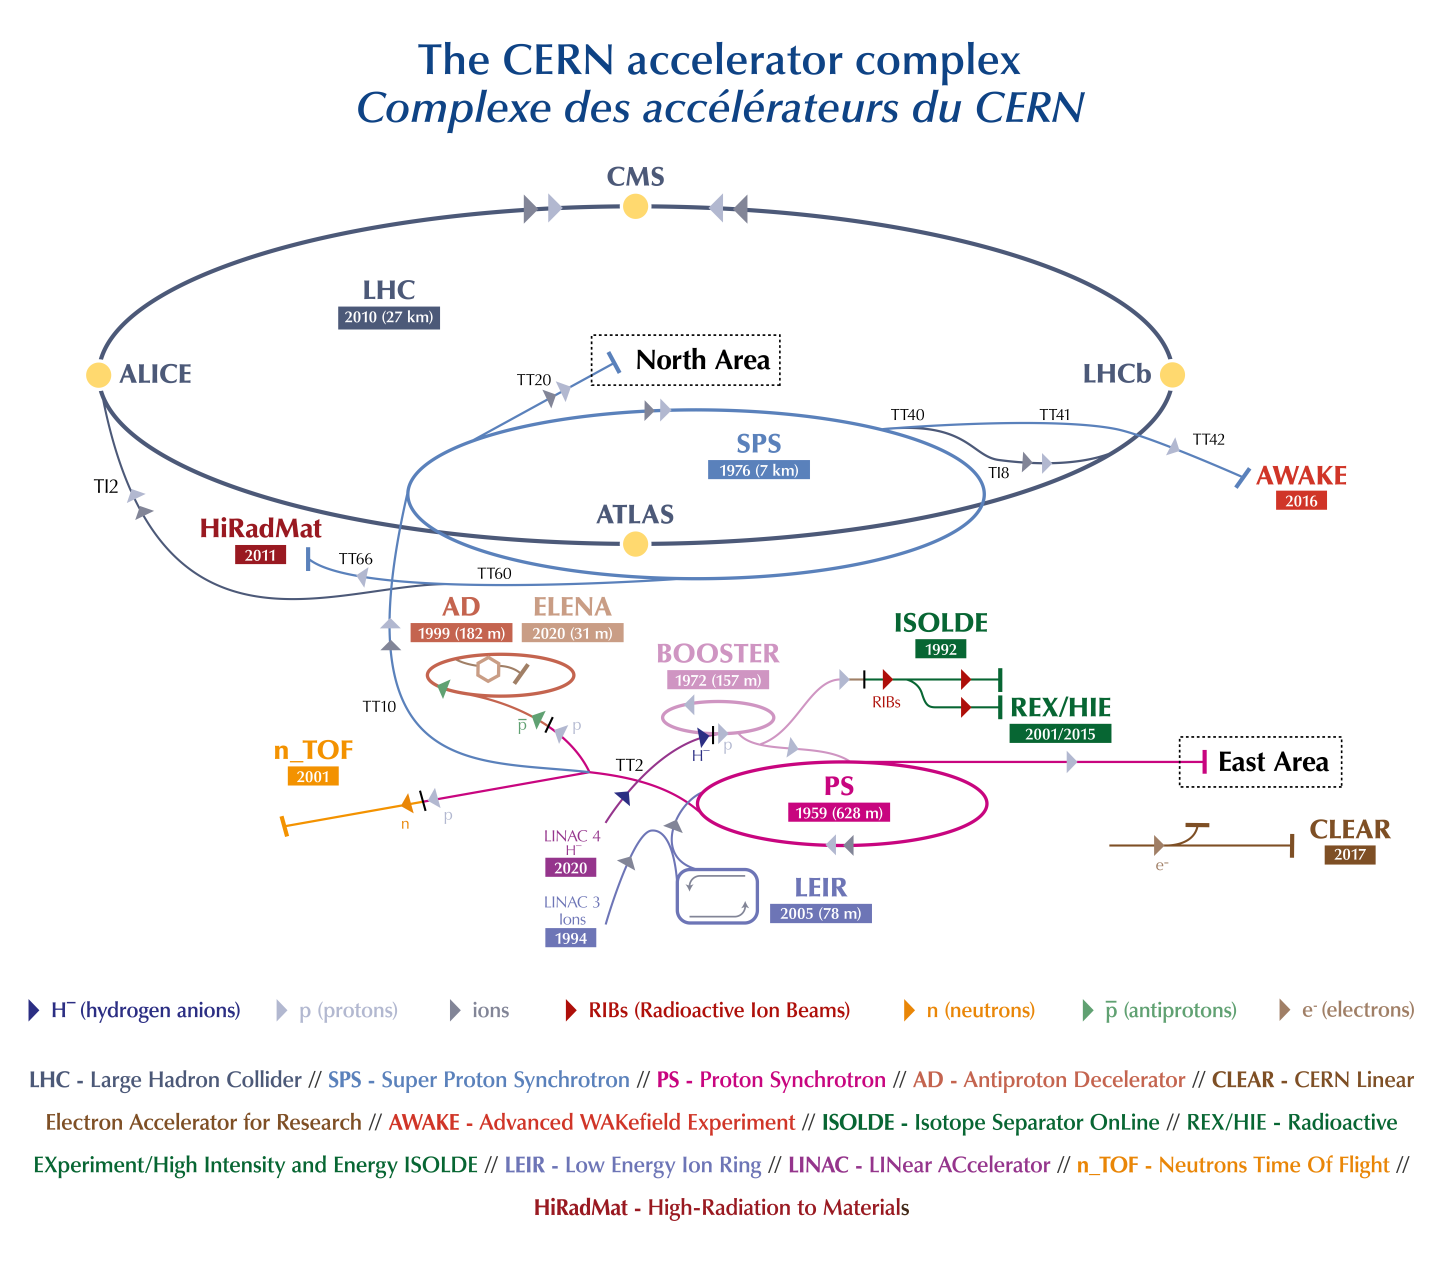
\includegraphics[width=0.9\textwidth]{Figures/LHC/CernAcceleratorComplex.png}
  \caption[The \CERN accelerator complex]%
  {The CERN accelerator complex, where the LHC is the largest ring. The four main collision points corresponding to the main experiments are dotted in yellow. This figure is from Ref.~\cite{Mobs:2684277}.}
  \label{fig:CERNComplex}
\end{figure}

The impressive feat of accelerating particles is made possible through the use of radio-frequency cavities. The idea was first crafted by the young Rolf Wideröe \cite{vretenar2012radio} for his PhD thesis and later caught the eye of the brilliant E. Lawrence, recipient of the Nobel Prize in Physics in 1939 for the invention of the cyclotron. RF cavities are round chambers along the beam. A voltage generator generate a voltage which oscillates at \unit{400}{\mega\hertz}, inducing an electric field inside the RF cavity. As particles pass through they experience the force of the field and are accelerated along the beam pipe. In total the LHC uses 8 RF cavities per beam (so 16 in total), with each cavity capable of delivering two megavolts (MV). Protons travelling through the cavity increase their energy to 14 times the injection amount, from 450 GeV to 6.5 TeV. Once protons get up to speed, a proton that has perfect timing will stay put, while protons that arrive slightly earlier/later will be accelerated/decelerate. The result is a beam of protons sorted into smaller segments of proton bunches. The LHC produces two such proton beams, one circulating clockwise and the other counterclockwise. 

A key concept in particle physics is luminosity. It is a factor that relates the cross-section to the number of event per second, written as follows:
\begin{equation}
    \luminosity=\dfrac{1}{\sigma}\cdot\dfrac{dN}{dt}
\end{equation}
where \luminosity is the luminosity, $N$ is the number of events, and $\sigma$ is the production cross section. The dimension of luminosity is events per unit time and unit area \unit{}{\cm\rpsquared}\unit{}{\second\rp}.

There are two properties used to describe a particle beam: its \todo{write more about this} emittance $\epsilon$, and its $\beta$ function. The emittance can be thought of as the area occupied by the particle beam in the position momentum plane. A lower emittance means the distance between particles and the difference in momentum between the particles are small. The cross sectional sizes of the beam $\sigma_i$ ($i=x,y$) are written as 
\begin{equation}
    \sigma_i=\sqrt{\dfrac{\beta_i\cdot\epsilon_i}{\pi}}
\end{equation}
The beams are assumed to be Gaussian distributed, meaning that in collisions, the centres of the beams contribute most while the edges have minimal impact. Following this the luminosity is
\begin{equation}
    \luminosity=\dfrac{N_1N_2f_{rev}N_b}{2\pi\Sigma_x\Sigma_y}
\end{equation}
where $N_1$ and $N_2$ are the number of particles for each bunch, $N_b$ is the number of bunches, $f$ is the revolution frequency, and $\Sigma_x,\Sigma_y$ represent the \unsure[]{Read more about this!} convolution of the beam sizes. They can be expressed as
\begin{equation}
    \Sigma_x=\sqrt{\sigma_{x1}^2+\sigma_{x2}^2}, \quad \Sigma_y=\sqrt{\sigma_{y1}^2+\sigma_{y2}^2}.
\end{equation}
Assuming that the beam sizes are identical and round, $\sigma_{x1}=\sigma_{x2}=\sigma_{y1}=\sigma_{y2}$, and the luminosity becomes
\begin{equation}
    \luminosity=\dfrac{N_1N_2f_{rev}N_b}{4\pi\sigma^2}=\dfrac{N_1N_2f_{rev}N_b\gamma}{4\pi\epsilon_N\beta^*}.
\end{equation}

When proton beams cross at the LHC, there are many collisions which occur other than the hard-scatter of interest. While increasing the number of particles per bunch increases the likelihood of a rare interaction, it also increases the pile-up of multiple interactions. Pile-up, denoted as $\mu$, is one of the biggest obstacles for LHC experiments; the more there is, the more difficult it becomes to disentangle the events of interest from the sea of low energy collision. It is, however, an inevitable consequence that accompanies increasing the instantaneous luminosity \todo{Write more about why int. lumi. is wanted to be high}. The contribution to pile-up events can be separated into two main categories: 
\begin{itemize}
  \item In-time pile-up refers to simultaneous proton-proton collisions occurring in the same bunch crossing as the hard scatter of interest;
  \item Out-of-time pile-up is the overlay of events from neighbouring bunches which contaminate signal events, attributed to detector electronics latency.
\end{itemize}
There are also less-substantial contributions from the cavern background, beam halo events, and beam gas events. The cavern background is the cloud of gas that floods the LHC cavern during operation. Beam halo events are from when the proton beam interacts with the collimating instrumentation, and the beam gas events describe interactions between the beam and the residual gas in the beam pipe. 

The \LHC was originally designed to reach a peak instantaneous luminosity and average pile-up of \unit{$10^{34}$}{\rpsquare{\cm}\reciprocal{\second}}\todo{Citation?} and $\langle\mu\rangle=19$ respectively. 

\begin{figure}
  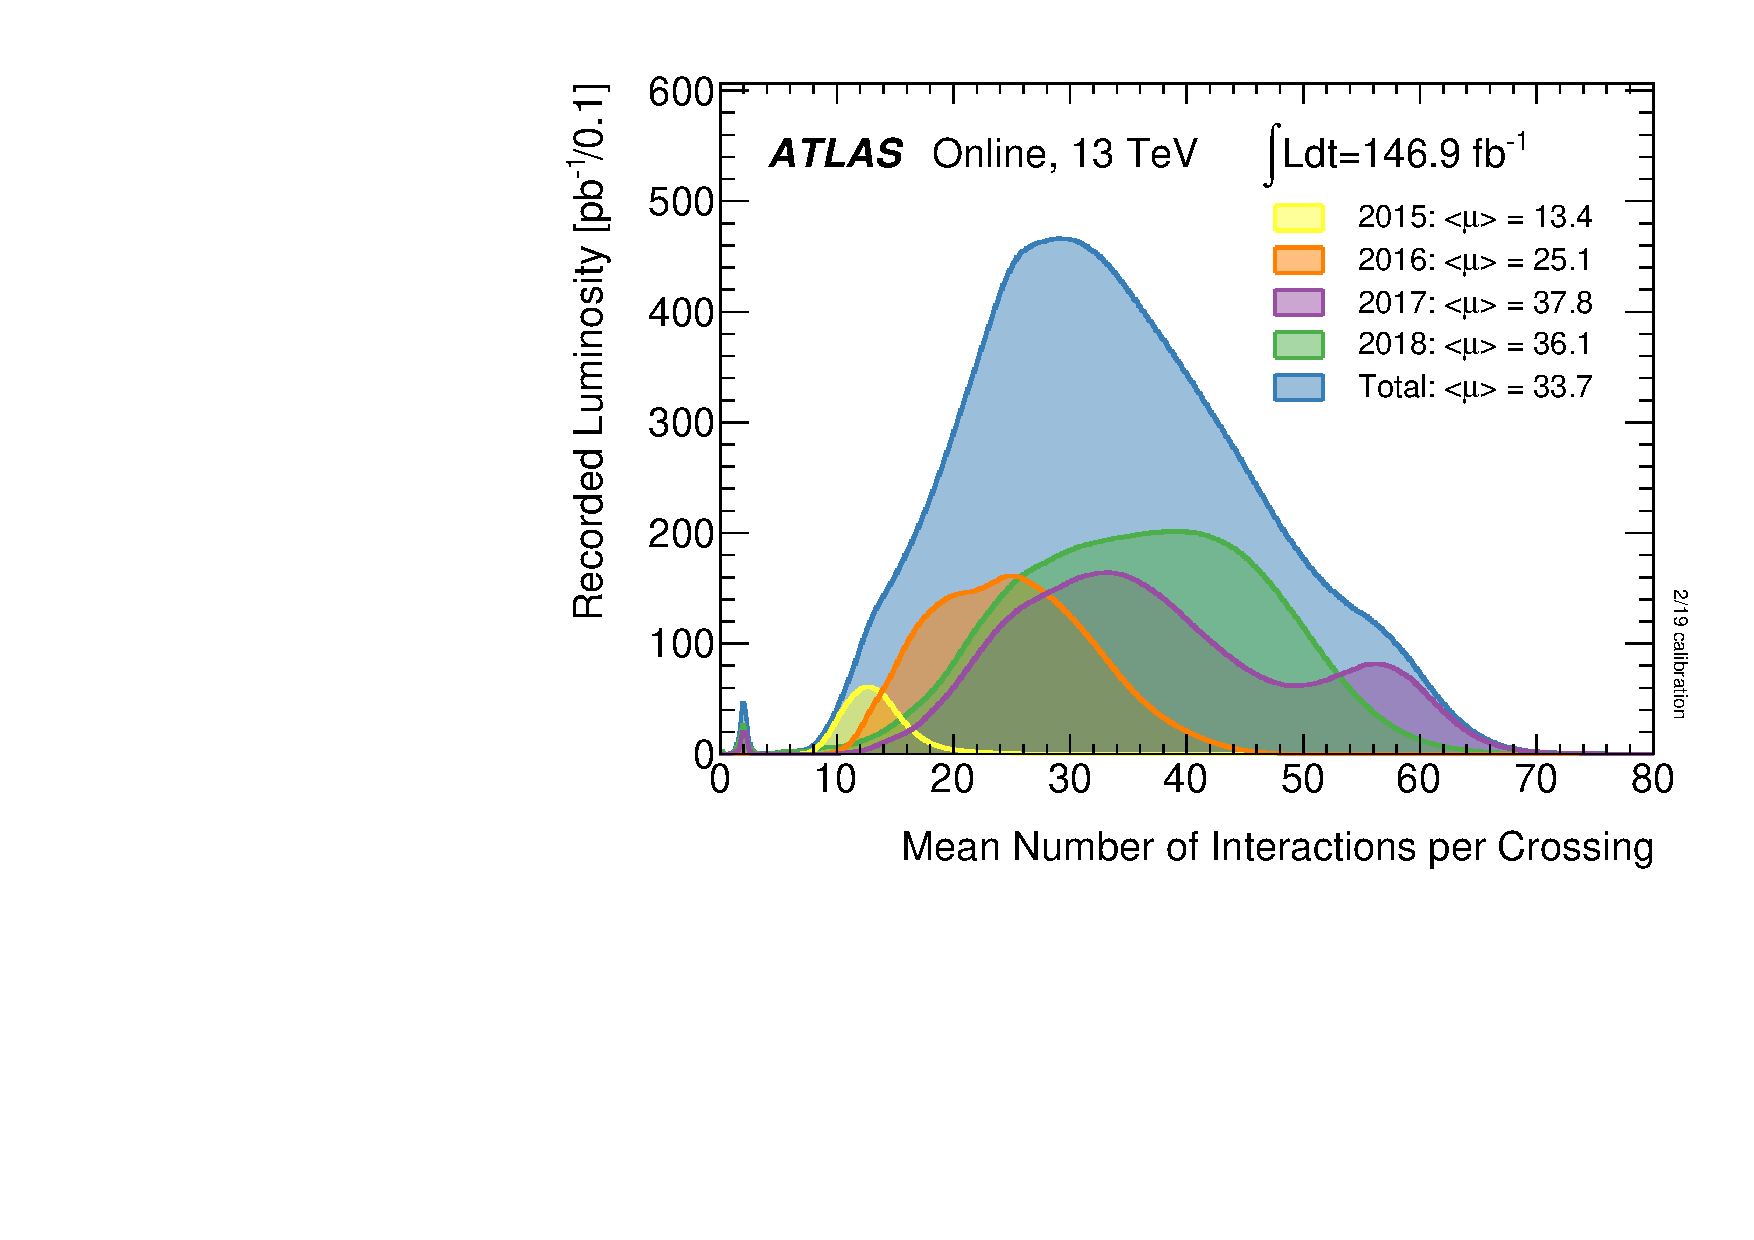
\includegraphics[width=0.7\textwidth]{Figures/LHC/PileUp_2015_2018.pdf}
  \caption[Pile-up distributions.]
  {The pile-up, $\mu$, is the mean number of collisions per bunch crossing. Shown is the \unit{13}{\TeV} are the pile-up distributions from 2015-2018, where each distribution is luminosity weighted. This figure is from Ref.~\cite{Boyd:2707815}.}
  \label{fig:Pileup}
\end{figure}

\section{The ATLAS detector}\label{sec:ATLAS}

Measuring forty-six meters in length, twenty five meters in height and width, and weighing in at a hulking seven thousand tons, the ATLAS (A-Toroidal-LHC-ApparatuS) detector is the Mount Everest of particle detectors. Built with a cylindrical and symmetric structure around the beam pipe, it's detection region covers nearly the entirety of the $4\pi$ solid angle of the collision point. \ATLAS is a general purpose detector, and combines a multitude of detector technologies to conduct searches for new phenomena, and to make high-precision measurements of the Standard Model.

The right-handed coordinate system used by the ATLAS detector, and also very commonly in particle physics, is illustrated in figure \ref{fig:atlascoordinate}. The $z$-axis is parallel to the beam pipe, the $y$-axis points vertically to the sky, and the $x$-axis points to the centre of the \LHC ring. The $xy$-plane is often referred to as the transverse plane, and the frequently encountered variables $p_T$ and $E_T$ refer to the momentum and energy in the transverse direction respectively. The azimuthal angle in the transverse plane is denoted as $\phi$, and polar angle $\theta$ denotes the angle offset from the beam pipe. Another commonly used coordinate is the rapidity, $y$, of an object:
\begin{equation}
    y=\dfrac{1}{2}\ln\dfrac{E+p_Z}{E-p_Z},
\end{equation}
where $E$ is the object's energy and $p_Z$ is the momentum in the $z$-direction. Rapidity differences are invariant
with respect to Lorentz boosts along the beam axis. This is the key reason why rapidities are so crucial in accelerator physics~\cite{daw2012}. Alternatively there is the pseudorapidity $\eta$ in the massless limit:
\begin{equation}
    \eta=-\ln\tan \dfrac{\theta}{2}.
\end{equation}
Both rapidity and pseudorapidity are more commonly used than polar angle $\theta$. The separation of two detected objects, $\Delta R$, is given by
\begin{equation}
    \Delta R=\sqrt{\Delta y^2+\Delta\phi^2},
\end{equation}
which is Lorentz invariant under a boost along the longitudinal (beam) direction.

The rest of this section will review the three sub-detectors of \ATLAS - the Inner Detector, the Calorimeter, and the Muon Spectrometer - as well as the Magnet System. A cross-sectional diagram illustrating the sub-detector systems is shown in Figure \ref{fig:atlasdetector}. The sub-detectors are made up on a concentric barrels that wrap around the beam pipe, and circular endcaps placed at either end of the barrels. The barrels are designed to detect the particles that travel through the central $|\eta|$ region, and the endcaps broadens the angular coverage for particles whose trajectories run close to parallel to the beam. 

\begin{figure}
    \centering
    \resizebox{.6\textwidth}{!}{
    \tdplotsetmaincoords{75}{50} % to reset previous setting
    \begin{tikzpicture}[scale=2.7,tdplot_main_coords,rotate around x=90]
 
     % variables
      \def\rvec{1.2}
      \def\thetavec{40}
      \def\phivec{70}
      \def\R{1.1}
      \def\w{0.3}
     
      % axes
      \coordinate (O) at (0,0,0);
      \draw[thick,->] (0,0,0) -- (1,0,0) node[below left]{$x$};
      \draw[thick,->] (0,0,0) -- (0,1,0) node[below right]{$y$};
      \draw[thick,->] (0,0,0) -- (0,0,1) node[below right]{$z$};
      \tdplotsetcoord{P}{\rvec}{\thetavec}{\phivec}
     
      % vectors
      \draw[->,red] (O) -- (P) node[above left] {$P$};
      \draw[dashed,red] (O)  -- (Pxy);
      \draw[dashed,red] (P)  -- (Pxy);
      \draw[dashed,red] (Py) -- (Pxy);
     
      % circle - LHC
      \tdplotdrawarc[thick,rotate around x=90,black!70!blue]{(\R,0,0)}{\R}{0}{360}{}{}
     
      % compass - the line between CMS and ATLAS has a ~12° declination (http://googlecompass.com)
      \begin{scope}[shift={(1.1*\R,0,1.65*\R)},rotate around y=12]
        \draw[<->,black!50] (-\w,0,0) -- (\w,0,0);
        \draw[<->,black!50] (0,0,-\w) -- (0,0,\w);
        \node[above left,black!50,scale=0.6] at (-\w,0,0) {N};
      \end{scope}
     
      % nodes
      \node[left,align=center] at (0,0,1.1) {Jura};
      \node[right] at (\R,0,0) {LHC};
      \fill[radius=0.8pt,black!20!red]
        (O) circle node[left=4pt,below=2pt] {CMS};
      \draw[thick] (0.02,0,0) -- (0.5,0,0); % partially overdraw x-axis and CMS point
      \fill[radius=0.8pt,black!20!blue]
        (2*\R,0,0) circle
        node[right=4pt,below=2pt,scale=0.9] {ATLAS};
      \fill[radius=0.8pt,black!10!orange]
        ({\R*sqrt(2)/2+\R},0,{ \R*sqrt(2)/2}) circle % 45 degrees from ATLAS
        node[left=2pt,below=2pt,scale=0.8] {ALICE};
      \fill[radius=0.8pt,black!60!green]
        ({\R*sqrt(2)/2+\R},0,{-\R*sqrt(2)/2}) circle % 45 degrees from ATLAS
        node[below=2pt,right=2pt,scale=0.8] {LHCb};
     
      % arcs
      \tdplotdrawarc[->]{(O)}{0.2}{0}{\phivec}
        {above=2pt,right=-1pt,anchor=mid west}{$\phi$}
      \tdplotdrawarc[->,rotate around z=\phivec-90,rotate around y=-90]{(0,0,0)}{0.5}{0}{\thetavec}
        {anchor=mid east}{$\theta$}
 
    \end{tikzpicture}
    }
    \caption{The coordinate system used at the LHC in the perspective of the CMS experiment. Figure taken from~\cite{coordinatesys}.}
    \label{fig:atlascoordinate}
\end{figure}

\begin{figure}[htb!]
    \centering
    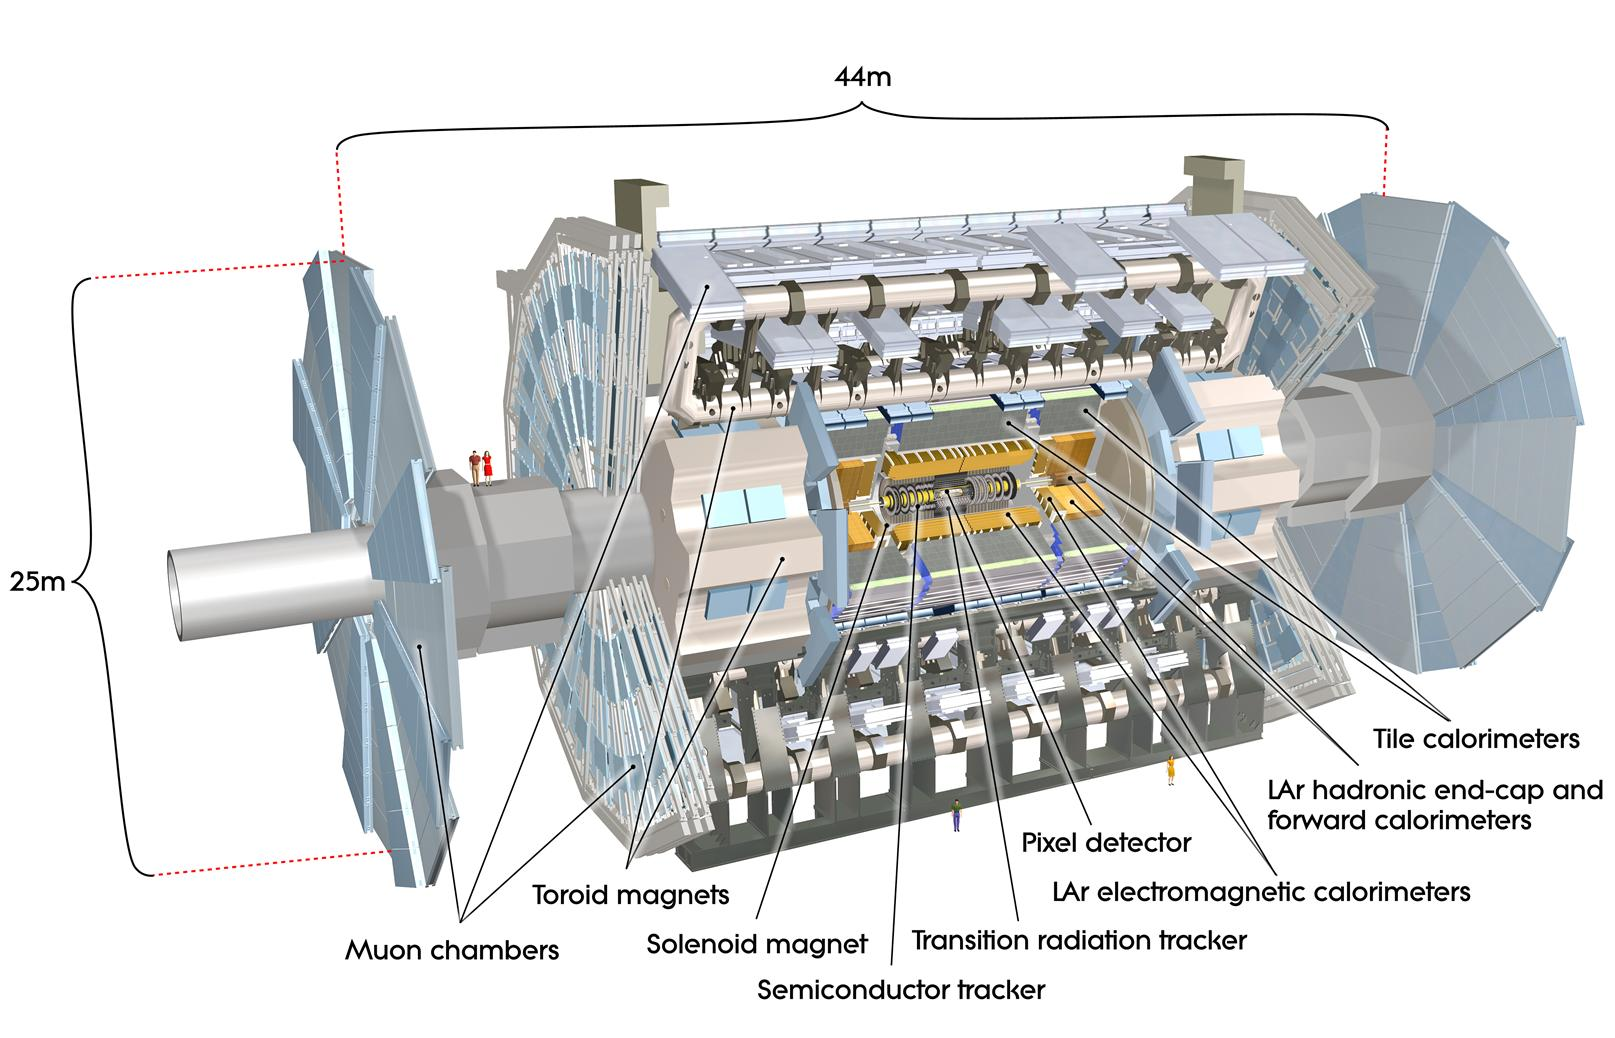
\includegraphics[width=0.99\textwidth]{Figures/LHC/ATLASDetector.jpg}
    \caption{The \ATLAS detector and its sub-components. This figure is from Ref.~\cite{Reed:2014}.}
    \label{fig:atlasdetector}
\end{figure}

\subsection{The Inner Detectors} \label{ssec:ATLASID}
The Inner Detector (ID) is able to measure the momentum of charged particles passing through it. The trajectories of the charged particles as they cross through are curved by a superconducting solenoid magnet with a 2 Tesla magnetic field~\cite{Yamamoto:1999}. The direction of curvature indicates the particle's charge, while the degree of curvature indicates momentum. The Inner Detector is the smallest component of ATLAS, stretching out to a radius of only 1.15 meters, with a total length of 7 meters. The barrel arrangement consists of concentric cylinders wrapped around the beam axis, and the end-cap components are attached as disks normal to the beam axis. The inner detector has three main components: the Pixel Detector, the Semiconductor Tracker (SCT), and the Transition Radiation Tracker (TRT).

\subsubsection{Pixel Detector}

The Pixel Detector is the innermost part of the Inner Detector. It is the part of ATLAS that is closest to the interaction point where particles collide. It was designed with extremely high granularity in mind in order to accurately resolve primary and secondary vertices, determine impact parameter resolution, and identify short-lived particles such as b-hadrons and tau leptons. Prior to Run 2, the pixel detector consisted of three concentric layers in the barrel, and three disks in the end-cap regions. During the long shutdown prior to Run 2, an additional layer called the Insertable B-layer (IBL)~\cite{Capeans:1291633} was added to the Pixel Detector closest to the beam pipe, making a total of four layers. The pixel detector are made up of sensor modules, each consisting of 46,080 active silicon pixels measuring 50 micrometers in width ($\phi$ direction) and 400 micrometers in length ($z$ direction). Each module consist of the active sensor medium (in this case silicon), and front-end electronics for readout. In total, the pixel detector hosts an astonishing eighty million readout channels. All together, the pixel detector achieves a resolution of \unit{10}{\micro\meter} in the $\phi$-direction and \unit{115}{\micro\meter} in the $z$-direction \todo{Check these numbers and cite}.

\subsubsection{Semi-conductor tracker}

The second layer of the inner detector is the SemiConductor Tracker (SCT), made up of two-sided modules of silicon microstrip sensors arranged back to back and tilted by a stereo angle of 40 mrad \cite{AHMAD200798}. It wraps around around the pixel detector and has in total 4088 modules, assembled in four cylindrical layers in the barrel region, and two end-caps containing nine disks each \cite{CERN-LHCC-2017-005}. The stereo angle enables the module to provide information about where along the strip the hit occurred. This is turn gives resolution in the z-plane in the barrels, and in R along the endcaps. The spatial resolution of the detector is \unit{17}{\mu\meter} in $R-\phi$ coordinate and \unit{580}{\mu\meter} in the $z$ coordinate in the barrel ($R$ in the endcaps) \cite{Abdesselam:974073}. In total the SCT hosts 4088 modules, assembled in four cylindrical layers in the barrel region, and two end-caps containing nine disks each \cite{CERN-LHCC-2017-005}. 

\subsubsection{Transition Radiation Tracker}

The third and outermost layer of the inner detector is the Transition Radiation Tracker (TRT). Unlike the ID and the SCT, it uses a straw drift tube technology, and exploits transition radiation emission for additional particle identification. Each module consists of 4 millimetre diameter straw tubes filled with xenon, carbon dioxide, and oxygen (70\%, 27\%, and 3\%)\cite{Vogel:1537991} bundled together. In order to collect charge from ionisation, a tungsten wire extends axially through the centre of each tube. In the barrel the drift tubes run parallel with the beam axis, and in the endcaps they run radially. In total there are 351,000 readout channels, and the resulting position resolution is weaker than the Pixel Detector or the SCT. The TRT is only capable of performing measurements in the $R-\phi$ coordinate, with a resolution of \unit{130}{\mu\meter}~\cite{Vogel:1537991}. 

Despite the lower resolution and the lack of sensitivity in the $z$ coordinate, the hits in the TRT contribute significantly to momentum resolution due to the a larger number of measurements and an extended measured track length. There are 73 parallel planes of straw-tubes in the barrel and 80 planes in each endcap. Furthermore, the barrel straws are inter-weaved in a matrix of polypropylene fibres, and the endcap disks are wedged in between polypropylene foils, creating numerous material boundaries. As highly relativistic particles pass through the boundaries they emit transition radiation photons; predominantly in the X-ray energy regime \cite{Ginzburg_1996}. These photons are absorbed by the gas mixture inside the tubes, and yield higher signal amplitudes than the signal of hits from minimum-ionizing particles. The energy of the transition radiation photon is strictly proportional to the relativistic factor $\gamma=E/m$ of the incident particle. For a given momentum, it is much higher for electrons than it is for pions or muons, a useful difference that is exploited for particle identification.

\subsection{Calorimetry}
Immediately after the particles exit the inner detector, they reach a set of calorimeters whose aim is to measure the particles’ energies by fully absorbing them. In contrast to the Inner Detector, the calorimeters can detect both charged and neutral particles. Neutrinos and muons, however, pass through the calorimeters unaffected as they are minimally ionizing particles (MIPs) at the LHC energy scale. The ATLAS calorimeters use sampling calorimeter technology. This is a design choice where layers of an active sensing material alternate with layers of a dense absorber material. Particles crossing the calorimeters will interact with the absorber medium and lose its energy through interactions. The initial traversing particle eventually creates a cascade of many lower energy particles - a particle shower. The sensitive detector medium sandwiched between will generate a signal proportional to this shower, with readout done through ionization or scintillation. 
There are two types of particle showers: electromagnetic and hadronic, depending on the nature of the source. Electromagnetic showers are primarily initiated by electrons or photons and develop mainly through Bremsstrahlung ($e\rightarrow\gamma e$) and pair production ($\gamma\rightarrow e^+e^-$), while hadronic interactions are more complex, developing through the strong interaction between the hadrons and the absorber material's nuclei. They differ radically, and thus require separate detector technologies for high-precision detection.  In order to meet these needs, there are two types of calorimeters that are hermetic along the $\phi$ coordinate and cover up to $|\eta| < 4.9$. As depicted in Figure \ref{fig:calorimeters}, these are the electromagnetic and the hadronic calorimeters. 

\begin{figure}
    \centering
    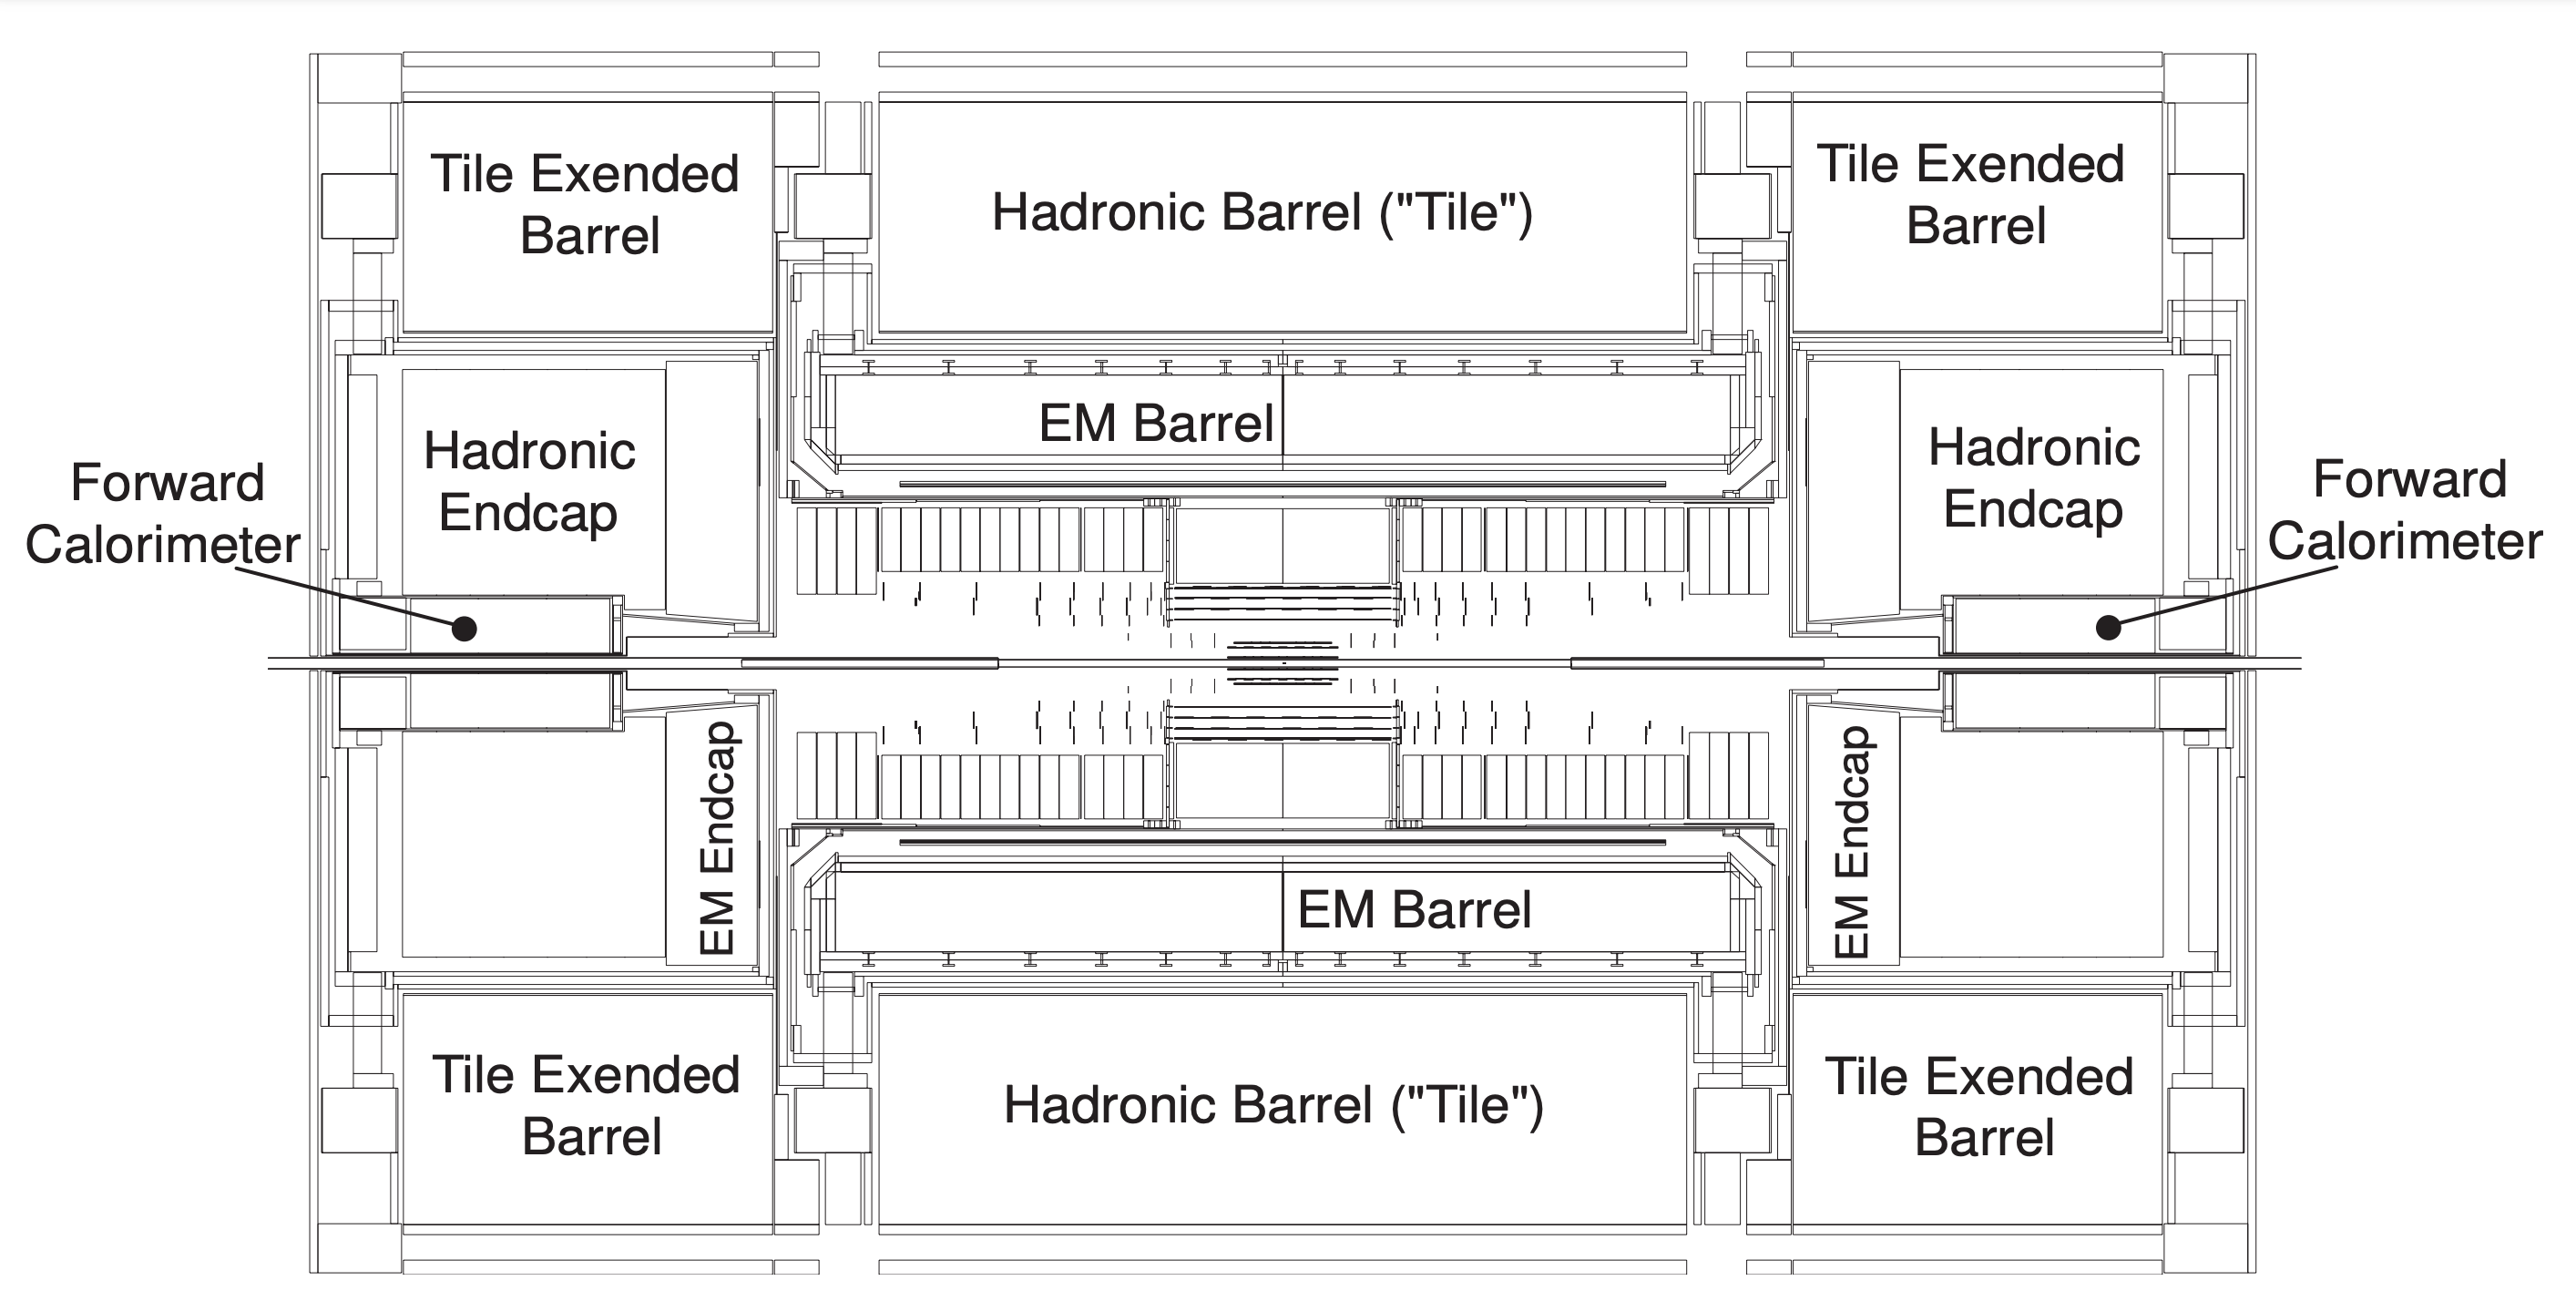
\includegraphics[width=0.99\textwidth]{Figures/LHC/ATLASCalorimetry.png}
    \caption{Cross-sectional view of the calorimetry system in the ATLAS detector. This figure is from Ref.~\cite{Lampl:923625}.}
    \label{fig:calorimeters}
\end{figure}

\subsubsection{The Electromagnetic Calorimeter}
The electromagnetic calorimeter wraps immediately around the inner detector as illustrated in Figure \ref{fig:calorimeters}. The material used for the active sensing medium is liquid Argon (LAr), chosen for its high intrinsic uniformity, long-term stability of signal response, as well as radiation hardness~\cite{Zhang_2011}. Lead plates are used as absorbers, chosen for it's high hadronic interaction length to radiation length ratio. The resulting electromagnetic calorimeter has a total thickness that covers twenty two times the radiation length, which corresponds to less that one hadronic interaction length, preventing hadronic showers from former. The liquid Argon and lead layers and arranged in an accordian-like geometry, ensuring a full azimuthal coverage with minimal gaps in acceptance \todo{Find a figure? Can't seem to visualise how this helps}. The barrel sector consists of three layers of varying granularity and has coverage up to $|\eta| < 1.475$. 

The first layer has a granularity of $\Delta\eta\times\Delta\phi=0.0031\times 0.098$. The high $\Delta\eta$ resolution acts as a powerful discriminator between showers originating from single isolated photons and those originating from multiple photons, from decays of neutral mesons within jets \todo{Read more about this}. The second layer is the thickest of the three, and it absorbs the vast majority of the shower's energy. It has a granularity of $\Delta\eta\times\Delta\phi=0.025\times 0.025$. Lastly, a thinner, lower-granularity final layer with $\Delta\eta\times\Delta\phi=0.05\times 0.025$ is used to estimate the energy that leaks beyond the electromagnetic calorimeter and into the hadronic calorimeter. In order to correct for energy lost by electrons and photons when they interact with the inner detector and magnet, a liquid Argon pre-sampler is installed upstream of the calorimeter. The pre-sampler is one single sensitive layer of liquid Argon and covers the range $|\eta| < 1.8$. The electromagnetic calorimeter end-caps are made up of four wheels; an inner and outer wheel on either side of the interaction point. These are each divided into eight wedge shaped modules and cover the range $1.375 < |\eta| < 3.2$. Like the barrel modules, the end-cal modules consist of three layers of varying granularity.

\subsubsection{The Hadronic Calorimeter}
Hadrons lose energy by through inelastic interactions with the detector medium, which result in the production of secondary strongly interacting particles, giving rise to hadronic showers\todo{Reword?}. The main purpose of the hadronic calorimetry system is to measure the energy such hadrons. Its performance is essential for precision measurements of jets as well as reconstruction of missing energy~\cite{Aaboud:2018scw}. The hadronic calorimeter incorporates modules of varying technologies, the barrel region hosts a tile calorimeter and the end-caps host a liquid-argon hadronic calorimeter. 

The Tile Calorimeter, covering the central region of ATLAS, is further separated into two sub-detectors. In the $|\eta| < 1.0$ region there is the hadronic tile barrel, and the extended tile barrel resides between $0.8 < |\eta| < 1.7$. Both regions use alternating tiles of steel absorbers and scintillating sensing elements, arranged parallel to the beam axis. A total of 64 modules wedge together to give full azimuthal angle coverage. In the transverse direction there are three layers of varying granularity. The first and second layers have resolution $0.1 \times 0.1$ in $\Delta\eta\times\Delta\phi$, and the third layer a coarser resolution of $\Delta\eta\times\Delta\phi = 0.2 \time 0.1$. As an ionising particle crosses the scintillating medium, ultraviolet scintillation light is produced. Using wavelength-shifting optical fibers, this light is collected and converted into visible light \todo{Why is it converted to visible light?}. Next it is guided towards photomultiplier tubes at the top of each module, where the optical signal is measured.

The hadronic end-cap calorimeter is a liquid argon sampling calorimeter, similar to the its electromagnetic counterpart. The coverage reaches the $1.5 < |\eta| < 3.2$ range in the forward region, where the more radiation resistant liquid argon technology is better suited than a tile calorimeter. The absorber in the hadronic end-cap, however, is copper rather than lead. Each end-cap consists of two separate wheels. The inner wheel has 8.5 millimetre liquid argon gaps wedged between 25 millimetre thick copper plates, whereas for the outer wheel the copper is 50 millimetre thick. The granularity is $0.1 \times 0.1$ in $\Delta\eta\times\Delta\phi$ for $1.5 < |\eta| < 2.5$, and $\Delta\eta\times\Delta\phi = 0.2 \times 0.2$ for $\Delta\eta\times\Delta\phi$ for $2.5 < |\eta| < 3.2$.

%%The Tile barrel measures 5.8 m in length, whereas the two extended barrels 2.8 m each. Both systems have an inner radius of 2.28 m and an outer radius of 4.25 m. 


\subsection{The Muon Spectrometer}
\label{ssec:ATLASMS}
The outermost layer of the \ATLAS detector system is the muon spectrometer, which as the name suggests, is designed to provide efficient, high-resolution measurements of muons' trajectory and momenta. Installing this tracking system wrapping around the other sub-detectors gives muons a very distinctive detector signature, leading to a high purity and efficiency in their reconstruction. Figure \ref{fig:muonspectrometer} shows the layout of the muon system, which consists of four gaseous tracking chambers installed between the eight coils of the barrel toroidal magnetic system, as well as before and after the toroid magnets of the endcaps. Two of these are precision tracking chambers made for precision momentum measurements, and the other two act as an efficient trigger system fast response \cite{PALESTINI2003337}. 

\begin{itemize}
    \item Monitored Drift Tubes (MDT): To provide precision coordinate measurements in the bending plane of the the muon spectrometer, Monitored Drift Tube (MDT) chambers are installed over the full pseudorapidity range $|\eta| < 2.7$. Each MDT component consists of a 3 cm diameter pressurised aluminium drift tube filled with 93\% argon and 7\% carbon dioxide gas at three bar \cite{LEVIN2008347}. As a muon passes through a drift tube, ionisation electrons drift towards the centre where a wire stretches through the longitudinal axis. 
    \item Cathode Strip Chambers (CSC): The number of MDTs is reduced in the forward region $2.0 < |\eta| < 2.7$, where particle flux is twenty times higher than the average in the rest of the MS. Here, Cathode-Strip Chambers (CSC) aid momentum measurement. The CSC are multi-wire proportional chambers, with the cathode segmented into strips, and the direction of the strip is perpendicular to one of the wires. This allows for two independent measurements of the muon: one for the ionisation electrons that are collected at the wire, the other one from the induced signal collected at the strips. \change[]{Read more about this} %reword, this is copy pasted.}
    \item Resistive Plate Chambers (RPC): Installed in the barrel region, these chambers provides fast tracking in the $\eta<1.05$ region. Each chamber is made up of two gaseous volumes, Bakelite plates, and read-out electronics \cite{PALESTINI2003337}. 
    \item Thin Gap Chambers (TGC): Installed in the endcaps, TGCs makes up the second part of the muon trigger system. In total each endcap has seven layers \todo{Is it 7 or 9 layers? Find a citation.} of TGC. Each layer is made up of two resistive grounded cathode planes, with a sheet of closely spaced wires sandwiched inside \cite{Etzion}. A positive high voltage is applied to the wire anode. The gap between the anode to cathode plane is thinner than the wire to wire spacing (\unit{1.4}{\milli\meter} and \unit{1.8}{\milli\meter} respectively), a characteristic reflected in the name of these chambers. TGCs act as a level-1 trigger, and provide high efficiency and excellent time resolution in a high-background environment \cite{NAGAI1996219}.

    %This feature in combination with a highly-quenching gas mixture of n-pentane and CO2 allows fast and safe operation at high particle flux. The signal read from the wires provides a bending direction position measurement with a few-mm accuracy. Copper strips separated from a graphite cathode plane by a flameresistant material layer provide an azimuthal measurement with a similar accuracy. 
\end{itemize}
\begin{figure}
    \centering
    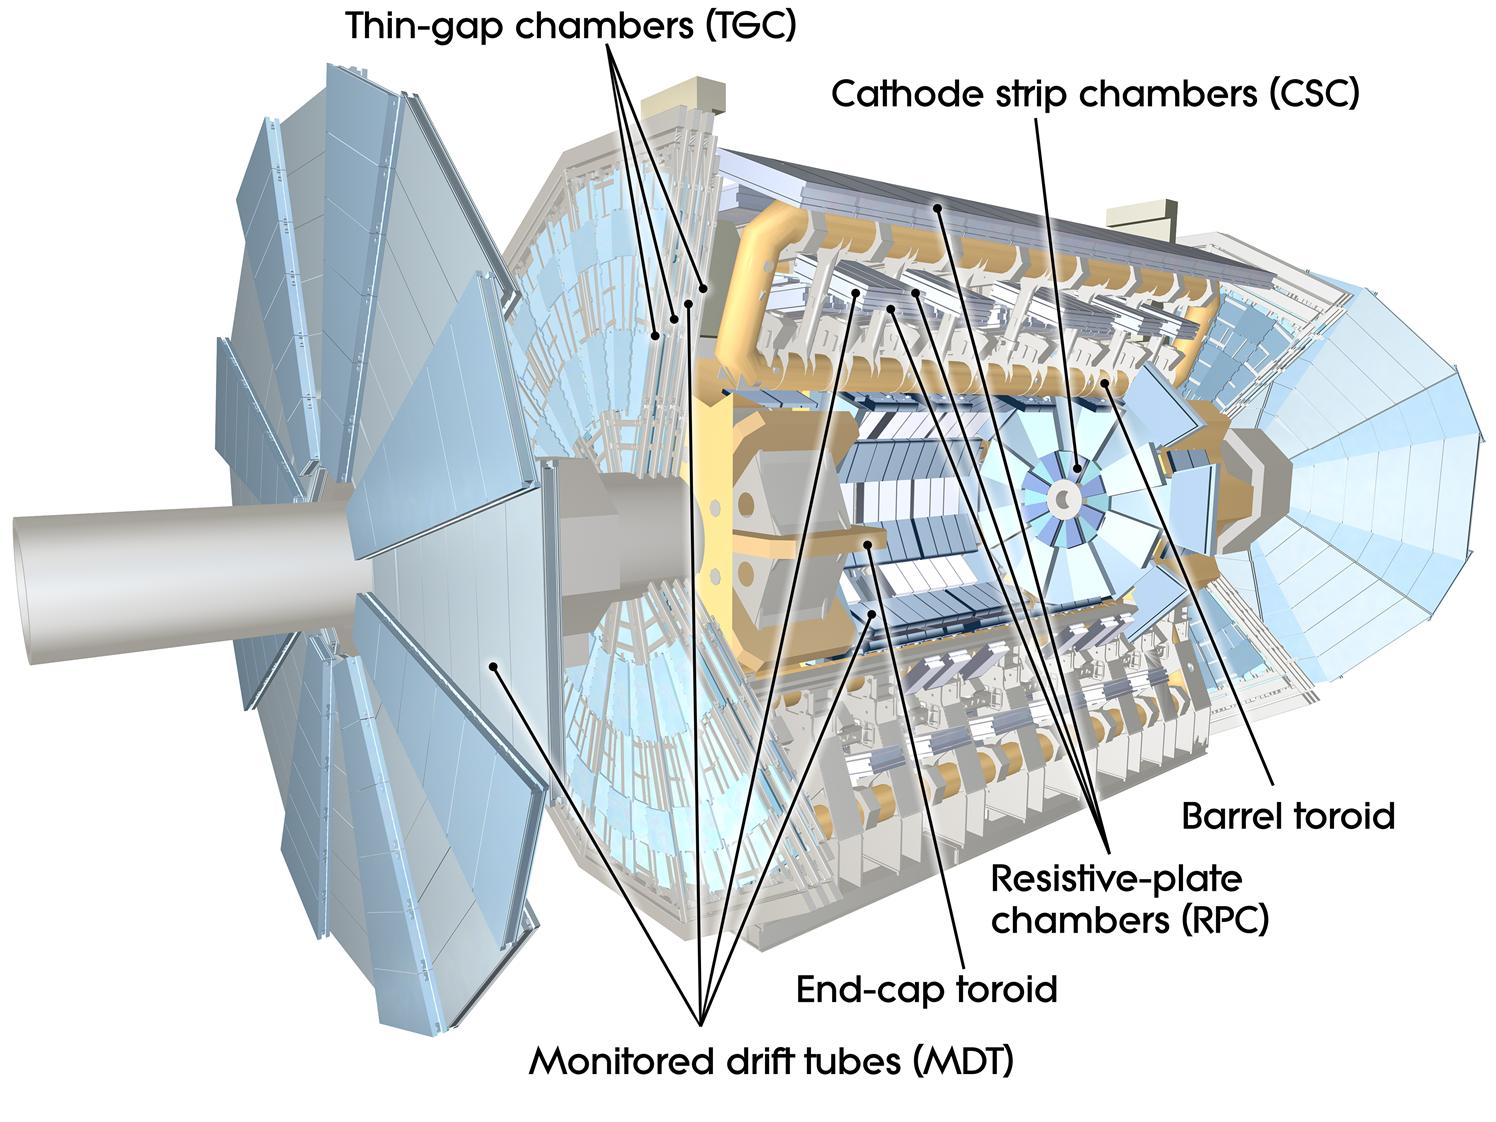
\includegraphics[width=0.8\textwidth]{Figures/LHC/ATLAS_MS.jpeg}
    \caption{A section view of the ATLAS Muon Spectrometer and its sub-components. This figure is from Ref.~\cite{ATLAS_MS}}
    \label{fig:muonspectrometer}
\end{figure}
\subsection{Magnet system}

The ATLAS detector incorporates a powerful magnet system that bends the trajectory of charged particles in order to measure their momentum with high accuracy. The momentum is deduced via the radius of curvature of the tracks seen within the detector systems. A pictorial representation of the ATLAS magnet system is shown in Figure \ref{fig:atlasmagnets}. It is a system comprised of four separate superconducting magnets - one barrel toroid and two endcap toroids incorporated in the muon spectrometer, and one central solenoid surrounding the inner detector. All four magnets are indirectly cooled, through conducting, by circulating helium at 4.5 K in the tubes welded onto the aluminum structure that encloses the coils \cite{828245}. 

The central solenoid is cylindrical in shape, and designed with minimal thickness in order to reduce energy loss before the particles enter the calorimeter. It is a superconducting magnet constructed from niobium-titanium alloy. It provides a magnetic field of \unit{2}{\tesla} to the inner detector axially (parallel to the $z-$axis), deflecting charged tracks along the $\phi$ coordinate. The strength of the central solenoid's magnet field is near constant along the radial direction, however it decreases on the axial edges due to the finite length of the magnet. 

The air toroid system is composed of three magnets: one forming a barrel section, and the others two end-caps. Each is composed of eight coils positioned in azimuthal symmetry around the beam axis. The toroids bend charged particles in the muon spectrometer. Unlike the central solenoid, however, the magnetic field strength varies. In the barrel it is between 0.15 Tesla and 2.5 Tesla, and in the endcaps it starts at 0.2 Tesla and reaches up to 3.5 Tesla \todo{Check these values and cite}. The toiroids' generated magnetic fields are orthogonal to that of the solenoid. This has the advantage that independent measurements of muon momenta can be made in the inner- and outer-most regions of the detector.

\begin{figure}[htb!]
    \centering
    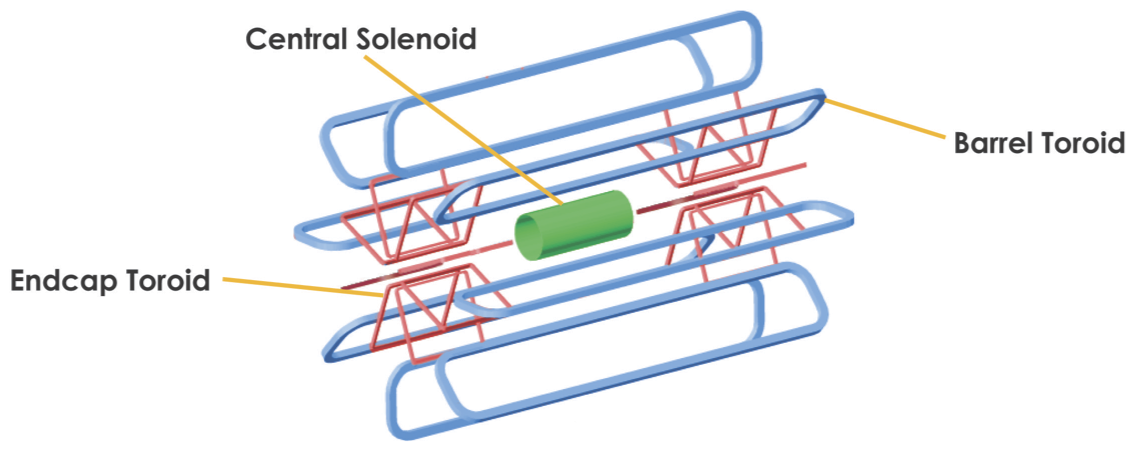
\includegraphics{Figures/LHC/exp-magnets.png}
    \caption{Schematic representation of the ATLAS magnet system. This Figure is from Ref.~\cite{atlasmagnet}.}
    \label{fig:atlasmagnets}
\end{figure}

\subsection{Trigger system}
\label{ssec:ATLAStrigger}
ATLAS does not record every single collision that the LHC produces. This is partially because most events are uninteresting low-energy processes, and partially because the amount of bandwidth and computing resources required make it impossible to do so. During run 2 the LHC had a bunch crossing rate of twenty five nanoseconds, corresponding to a collision frequency of forty megahertz. That's on the order of a few thousand gigabytes of data per second! It is neither feasible or practical to read out and record data at this frequency, and here the nifty trigger system comes into play. The ATLAS triggers act like a fine sieve and selects only rare, interesting events. Typically, interesting events involve objects that have high momentum or energy in the transverse direction. The ATLAS trigger system throughout run 2 effectively reduces the crossing rate from forty megahertz to one kilohertz through two triggers. The first is the level-1 (L1) trigger, a hardware based trigger that uses coarse objects from the calorimeters and the muon spectrometer, which reduces the rate to 100 kilohertz. The second is a software based high level trigger (HLT), which makes further selection choices bringing the final rate to one kilohertz. 

\subsubsection{Level-1 trigger}

The level-1 trigger consists of several subsystems. The level-1 calorimeter (L1Calo) and level-1 muon (L1Muon) subsystems operate separately with calorimetry and muon spectrometry information. The L1Calo trigger receives reduced resolution analogue signals from calorimeter trigger towers. These are formed by $\eta\times\phi=0.1\times0.1$ regions in the barrel and $\eta\times\phi=0.4\times0.4$ regions in the endcaps~\cite{pdg_2021}, separately for the electromagnetic and the hadronic calorimeter~\cite{Aad:2716326}. In the central region $|\eta| < 3.2$, L1Calo uses a sliding window algorithm to search for local maximum and forms regions of interests (ROIs) around them, which are sent for further processing to the HLT. L1Muon looks for coincident hits in the muon spectrometer; more specifically in the resistive plate chambers of the barrel region and and thin gap chambers in the endcaps, see Section~\ref{ssec:ATLASMS}. Finally there is the level-1 topological trigger (L1Topo), which makes use of takes trigger objects from both L1Calo and L1Muon and combines them into topological information. For example, one can require that two leptons have small angular separation $\Delta R < 0.1$. The L1 trigger makes a binary accept or reject decision via the the central trigger processor (CTP) which takes input from the three L1 subsystems. The acceptance rate reaches up to \unit{100}{\kilo\hertz}, and the data latency is \unit{2.5}{\micro\second}. 

\subsubsection{High level trigger}

Once the level-1 trigger has accepted an event, it passes the baton onto the software-based high level trigger (HLT) for processing. The HLT uses the ROIs provided by the L1 trigger to seed regional event reconstruction with full detector granularity, including tracking information from the inner detector. Upon receiving an accept signal from the L1 trigger, the front-end electronics sent data out to the readout system via readout drivers \todo{what does readout driver do?}. Reconstructing events is computationally expensive, thus the HLT is a built as a series of numerous individual trigger chains. At each stage an event may be rejected should it fail to meet the criteria of the chain. Rejected events are aborted, avoiding the need to run more CPU intensive algorithms. Once the HLT decides to accept an event, the full event data from various detectors are gathered and transferred to the tier-0 facility at CERN for preliminary analysis. The final event acceptance rate is reduced to \unit{1}{\kilo\hertz}, a much more bearable 300 megabytes per second. 

\todo[inline]{Write a bit about fast tracker? See http://cds.cern.ch/record/2633492/files/ATL-DAQ-PROC-2018-017.pdf}

% The Fast TracKer (FTK) [8] is a fast hardware-based track trigger system for ATLAS designed to perform a global track reconstruction receiving input from the silicon tracking detectors (part of the Inner Detector, ID) after each L1 trigger (at a rate of up to 100 kHz) and provide full-event track information to the HLT. The FTK aims at improving the efficiency of trigger selections that require tracking information, such as those to identify medium-pT b’s and τ’s, with high background rejection. Both b-tagging and τ identification rely on track information, as the former are characterized by a displaced vertex that can be reconstructed from the tracks in the event, and the latter have significantly less tracks in a smaller cone than standard jets. This is especially important for measurements where b-jets and third generation leptons play a crucial role, such as Higgs coupling measurements or searches for particles predicted by BSM models. In addition to the physics gains, using FTK information in the HLT decision process can improve many trigger algorithms, in particular those relying on isolation variables (lepton triggers) and calorimeter information (jet and E miss T triggers), which are both affected by pile-up effects that be mitigated using FTK tracks

\section{Object reconstruction}

The \ATLAS detector's raw readout signals must be translated into meaningfiul physics information before delivered to analysis teams. The responsibility for this task falls upon the offline reconstruction system, which combines information from all sub-detectors to reconstruct and identify particles with the highest possible efficiency. 

\subsection{Tracks and vertices}
\label{ssec:tracksandvertices}

Reconstruction of complex physics objects, such as electrons and muons, begins with the construction of more basic inputs such as tracks, vertices, and calorimeter clusters. 
Charged particle trajectories are called tracks, and their reconstruction is crucial for many reasons. They are explicit inputs in the identification, reconstruction and isolation of electrons and muons, which is the signal process for the analysis of this thesis. The basic building block of a track is the detection of a signal above threshold, a hit, in the inner tracking detectors. In the pixel detector and semi-conductor tracker, the hits are first assembled into clusters of energy deposits that share common corners and edges, called space points. Tracks are seeded with a triplet of space points, and are extended by matching subsequent pixel and SCT hits using a Kalman filter \cite{ATLAS-CONF-2012-042}. 

When describing a track, five parameters are used: $d_0$ and $z_0$, the transverse and longitudinal impact parameters, $\phi$ and $\theta$, the azimuthal and polar angle, and $q/p$ describing the charge~\cite{Akesson:973401}. Together these are known as the perigee parameters. The two impact parameters are illustrated in figure \ref{fig:impactparameters}. The transverse $d_0$ is the transverse distance from the primary vertex to the point of closest approach in the $\eta-\phi$ plane, while the $z_0$ is the distance  from the $z-$axis. 
\begin{figure}
    \centering
    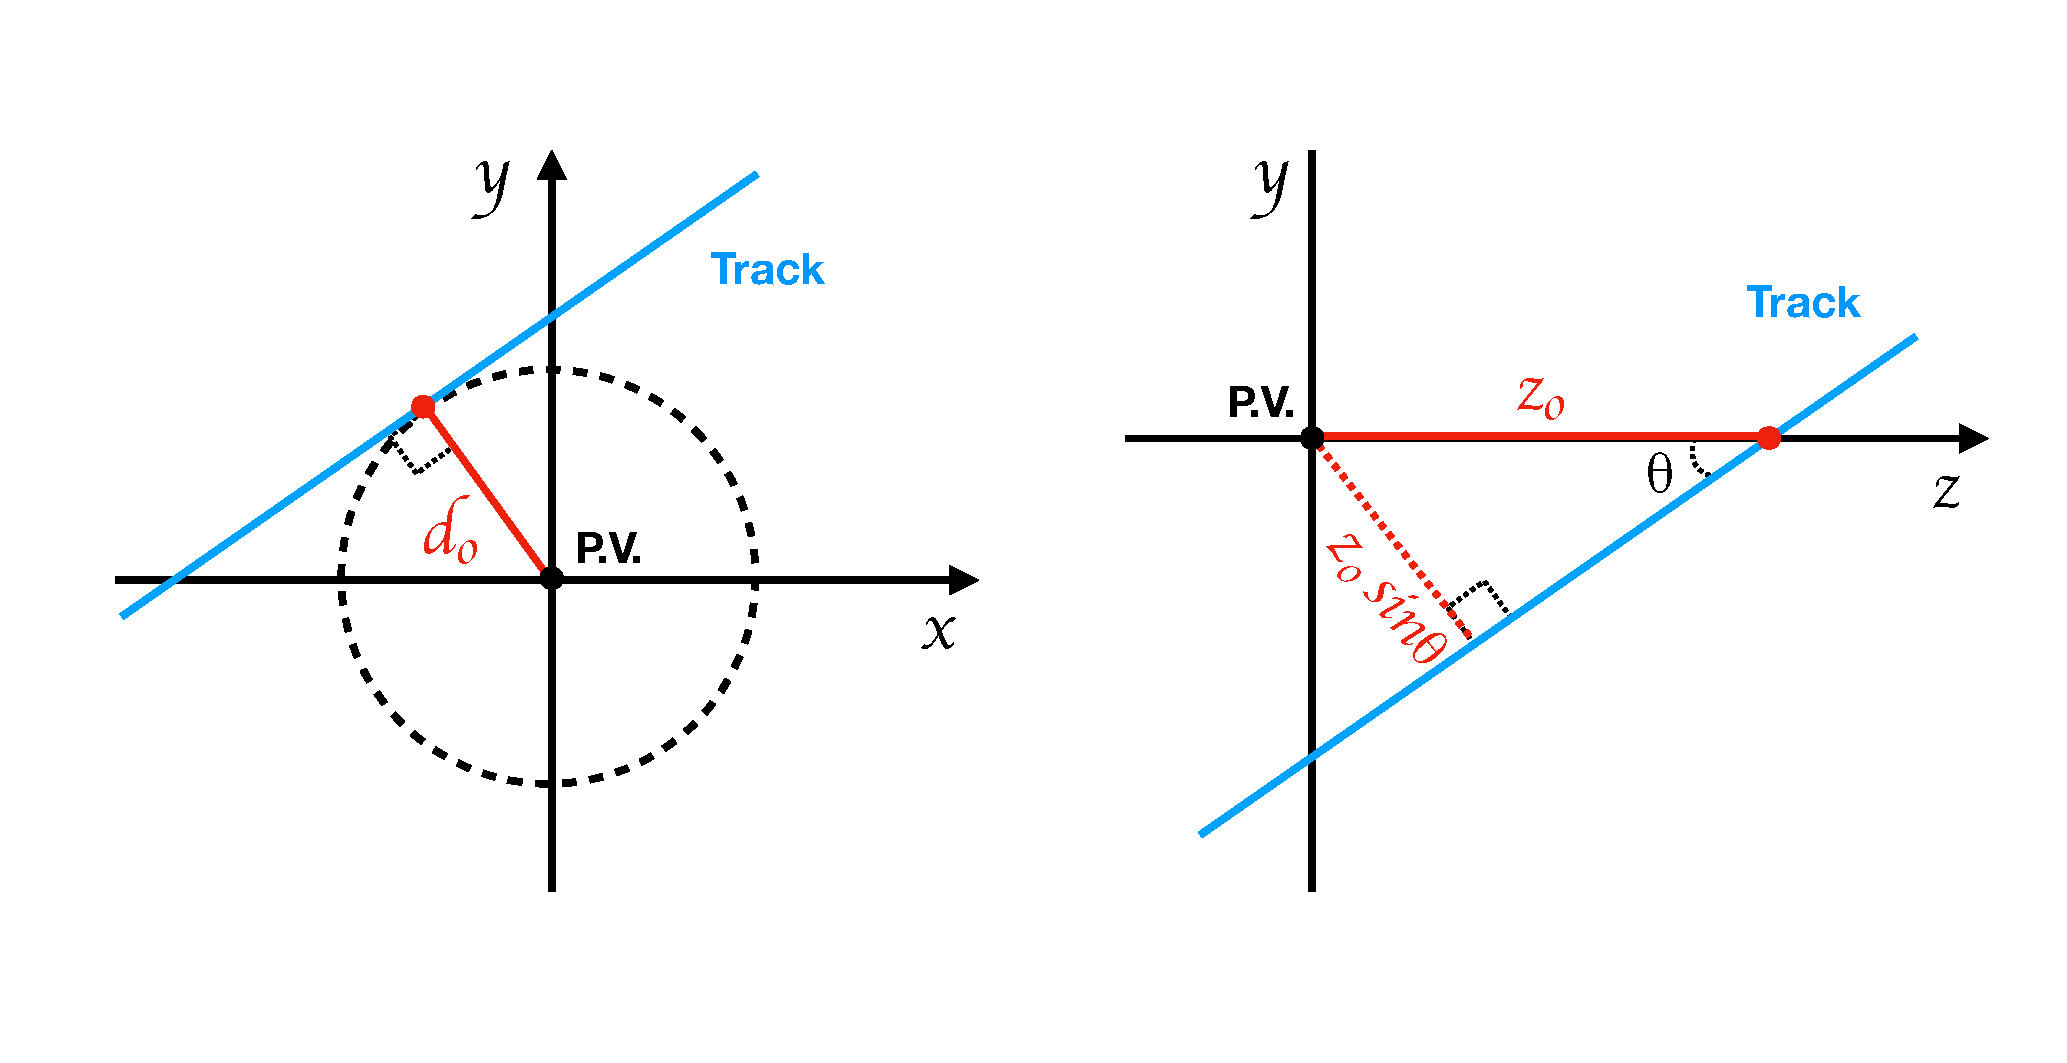
\includegraphics[width=\textwidth]{Figures/LHC/impact_params.pdf}
    \caption{Drawn in blue is the particle track, with the transverse and longitudinal impact parameters illustrated on the left and right graph respectively. The primary vertex (P.V.) is defined to be at the origin.}
    \label{fig:impactparameters}
\end{figure}
The momentum can be deduced from the track using the radius of curvature and the solenoid field strength. High momentum particles have less curved trajectories than low momentum particles. The collision vertex is the intersection of multiple particle trajectories at their origin. For vertex finding at least two reconstructed tracks are required as input. The primary vertices are points in space where proton–proton interactions have occurred \cite{ATLAS_primary_vertices}. Track to vertex association is split into two stages: 
\begin{itemize}
    \item Vertex finding associates reconstructed tracks to potential vertex candidates
    \item Vertex fitting is the reconstruction of the vertex position, as well as an estimate on the quality of the fit \cite{Piacquadio_2008}.
\end{itemize}
These two steps are often interlaced in the algorithms. With a set of selected tracks and a vertex seed position, an iterative procedure is used to find the best vertex position. After the vertex position is computed, incompatible tracks are removed and regrouped with the non-selected tracks to be used in finding and fitting or another vertex. 

\subsection{Clustering algorithms}
\label{ssec:clusteringalgorithms}
In the calorimeters, the signals are collected into related clusters. This is done to extract the significant signal coming from the hard scattering process from the noise \cite{Aad_2017_topo_clustering}. In the calorimeters, the noise arises from two main sources: the readout electronics, and pile-up from non-primary interactions \cite{Lampl:1099735}. The clustering algorithms aim to group together the calorimeter cells, in three dimensions, in which incoming particles have deposited their energy. The clustering allows for the computation of the sum of the total energy deposited. Within \ATLAS, there are two clustering algorithms: the sliding-window algorithm, and the topological algorithm. Both are summarised below and are described in detail in reference \cite{Lampl:1099735}. 

\subsubsection{Sliding-window algorithm}

The sliding-window algorithm first divides the $\eta-\phi$ space into a grid. All longitudinal cells' energies in each grid element is summed together to form rectangular prisms called towers. Next, a fixed sized window of $N_{\eta}\times N_{\phi}$ towers is used to scan across the grid in search of a local maximum above a chosen energy threshold. once found, it is used as a seed for the final step; cluster formation. Depending on the hypothesised particle type and the location in the calorimeter, the clusters pre-defined size in $\eta-\phi$ space varies \cite{Lampl:1099735}. Clusters are built by summing the energies of all cells within the defined size.

In cluster formation, the sliding window algorithm can form overlapping clusters if they share common cells. In these cases, the reconstruction algorithm (by default) includes the overlapping cells in both clusters, thus resulting in a double count of the energies of the shared cells. The disadvantage of this approach is that objects can be reconstructed with a larger energy that it had initially, due to the double counting. 

\subsubsection{Topological clustering}

Unlike the sliding-window algorithm, topological clustering results in clusters that have variable cell sizes. The building of clusters starts by examining the cell signal significance $\zeta_{\text{cell}}$, defined as
\begin{equation}
    \zeta_{\text{cell}} = \dfrac{E_{\text{cell}}}{\sigma_{\text{noise,cell}}}
\end{equation}
where the numerator is the energy deposited in the cell and the denominator is the average expected noise in the cell \cite{Aad_2017_topo_clustering}. In building the topological clusters, three thresholds are defined. The seed threshold $\zeta_{\text{seed}}$, the neighbour threshold $\zeta_{\text{neighbour}}$, and the baseline cell threshold $\zeta_{\text{base}}$. Any cell whose cell significant is above the seed threshold is labelled as a seed cell, and forms a proto-cluster. The seed cells are ranked from high to low based on their $\zeta_{\text{cell}}$ value. From there, neighbouring cells that have not been used as a seed cell are added to the proto-cluster if their energy is above $\zeta_{\text{neighbour}}$, and also added to the neighbour seed list. If a neighbour cell is next to two proto-clusters, then the proto-clusters are merged. If $\zeta_{\text{cell}}$ is below $\zeta_{\text{neighbour}}$ but still above $\zeta_{\text{base}}$, then the cell is added to the nearest neighbouring proto-cluster. After the original seed list is processed, it is discarded and the same procedure is repeated for neighbour seed list. This is done until no cells remain unprocessed. 

The advantage to the topological clustering method, as opposed to the sliding window method, is that it allows for a more organic growth of clusters rather than pre-defining its size and shape. The algorithm is formed so that it closely traces the spatial signal-significance
patterns generated by particle showers \cite{ATL-PHYS-PUB-2017-022}. Furthermore, topological clustering requires smaller energy loss corrections. It has a very efficient energy resolution and collects more energy on average than sliding window clustering \cite{ATL-PHYS-PUB-2017-022}. It is more complex to implement, however, and due to the dependency on noise levels, uncertainties from the electronics and pile-up directly affect the algorithm's reconstruction efficiency \cite{Lampl:1099735}. 

In reference \cite{ATL-PHYS-PUB-2017-022}, a topological clustering algorithm for electron and photon reconstruction is presented. It is demonstrated that this algorithm improves the energy resolution when compared to the traditional sliding window method. Figure \ref{fig:H4l_topo_cluster} shows the resolution improvements in the \HFourL channel, taken from reference \cite{ATL-PHYS-PUB-2017-022}. The topological cluster approach has a more narrow Higgs peak, and the peak is also closer to the true Higgs mass. After performing a fit with a double Crystal Ball function, the $4e$ channel shows a 5\% improvement in resolution.
\begin{figure}
    \centering
    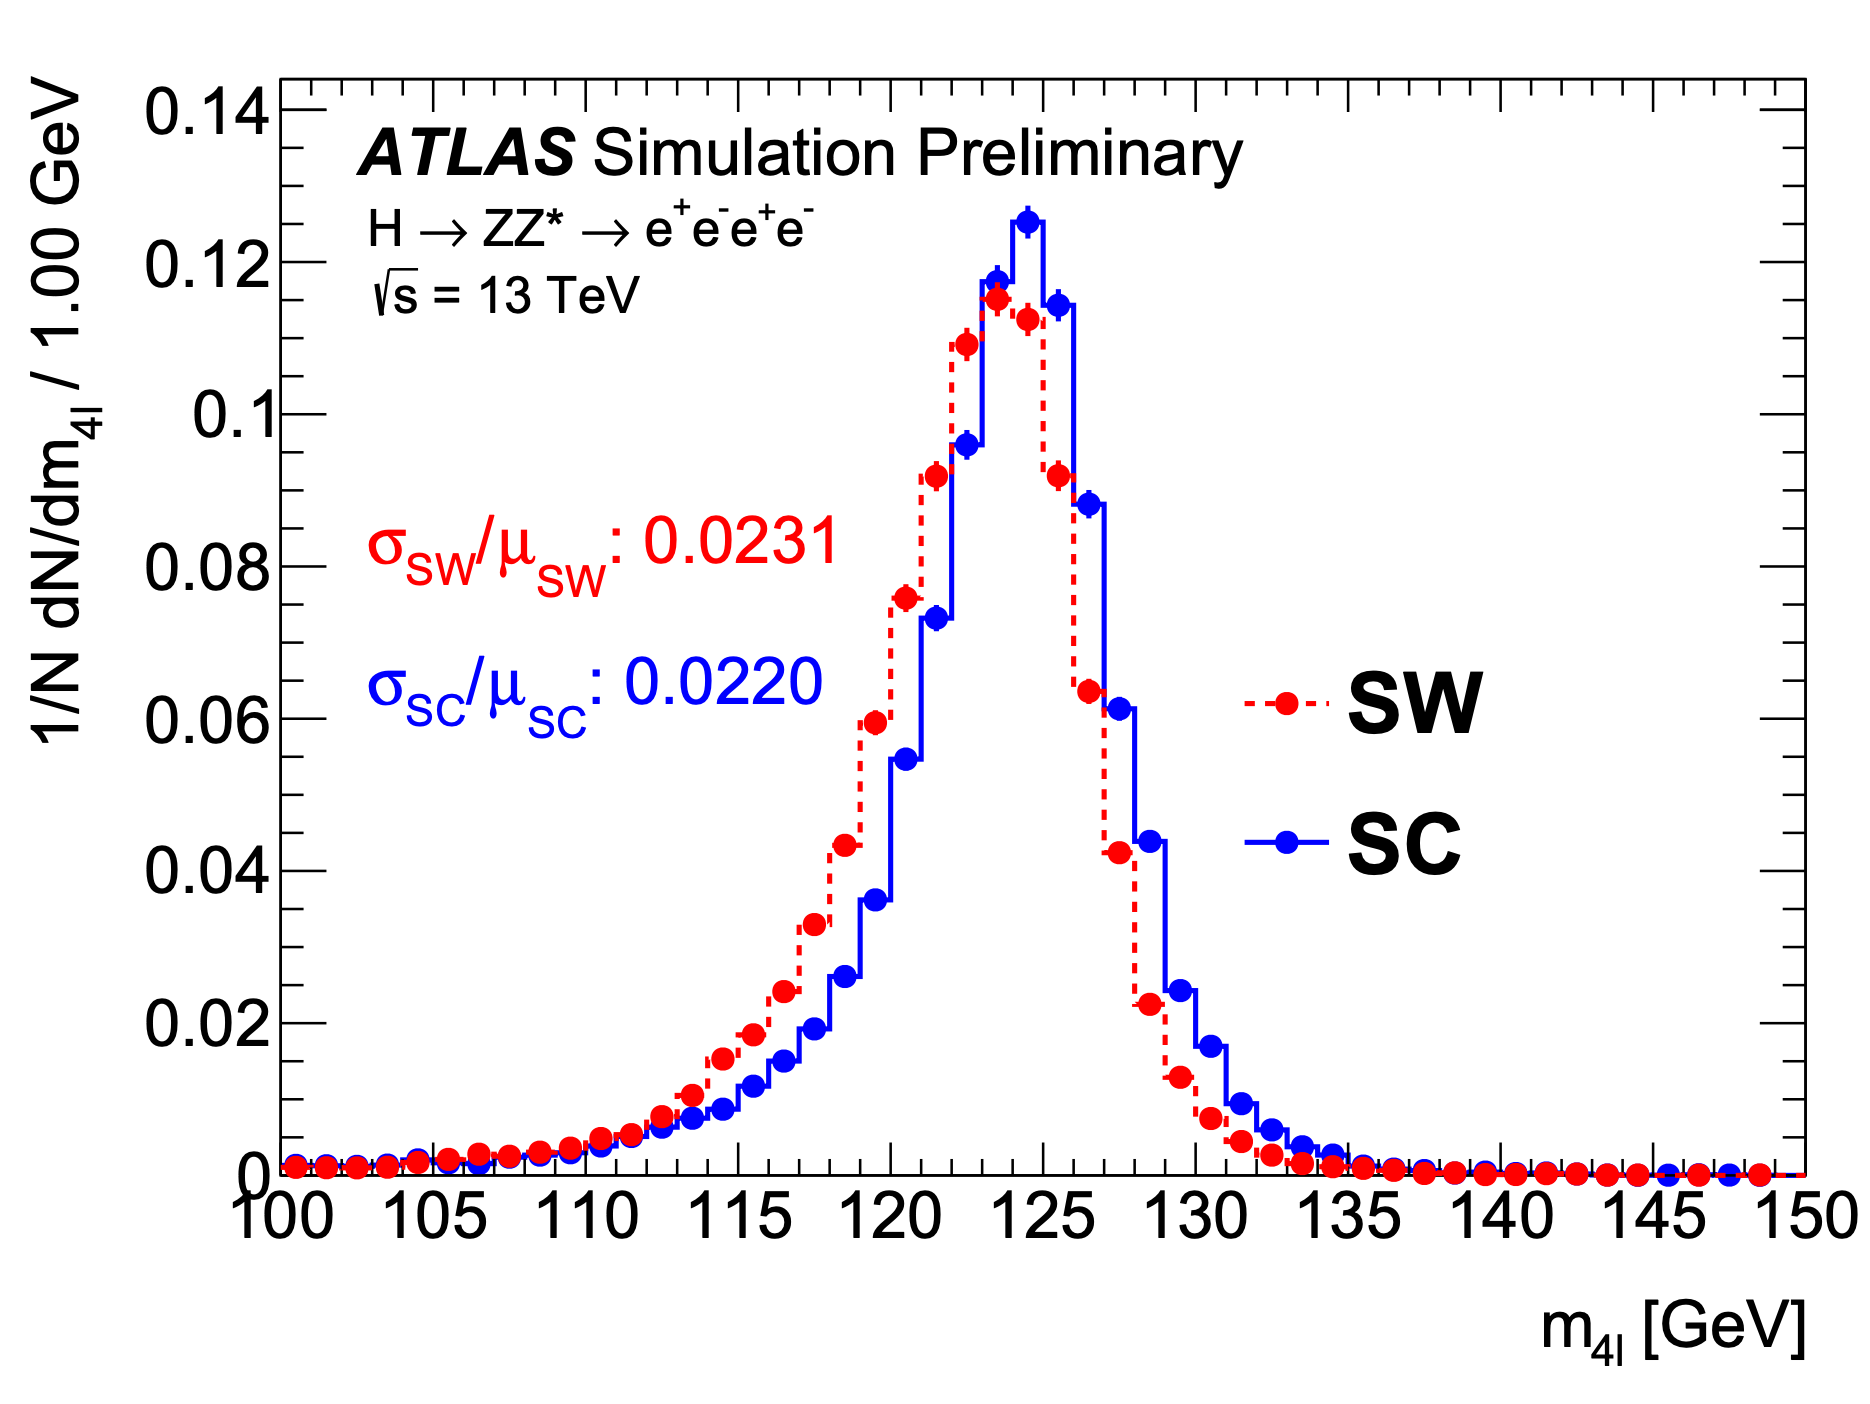
\includegraphics[width=\mediumfigwidth]{Figures/LHC/H4l_topo_cluster.png}
    \caption{Simulated 4 lepton invariant mass distributions using the supercluster and sliding window algorithms, in the $4e$ channel. This figure is from Ref.~\cite{ATL-PHYS-PUB-2017-022}.}
    \label{fig:H4l_topo_cluster}
\end{figure}

\subsection{Electrons}
\label{ssec:electronreco}
\subsubsection{Electron reconstruction}

Following track candidate and calorimeter cluster candidate reconstruction as described in sections \ref{ssec:tracksandvertices} and \ref{ssec:clusteringalgorithms} comes the final procedure in electron reconstruction: the matching of a track candidate to a topo-cluster and the finalisation of the cluster size \cite{ATLAS_electron_efficiency_2015-2016}. The algorithm prepares for reconstruction by first selecting the topo-custers and tracks it will use. The tracks are then refitted  using a Gaussian sum filter (GSF) method \cite{ATLAS-CONF-2012-047} to accommodate for the energy loss due to bremsstrahlung radiation, which affects electrons more significantly than muons due to their lighter mass. As an electron loses its energy, its transverse momentum also decreases, and the curvature of its track becomes more prominent. The refit improves electron reconstruction efficiencies by correcting for this effect and improving the track parameters.

By extrapolating the track from the perigee to the second calorimeter layer and using the track's momentum, re-fitted tracks are matched to topological clusters. Sometimes the momentum of the track is rescaled to match the energy of the cluster, which improves matching accuracy for electron candidates that lose a portion of their energy to bremsstrahlung radiation \cite{ATLAS_electron_efficiency_2015-2017}. In order for a track to match, the requirements $|\Delta\eta|<0.05$ and $-0.10<q\cdot(\phi_{\text{track}}-\phi_{\text{cluster}})<0.05$ must be fulfilled, where $q$ is the charge of the track. The asymmetry of the latter requirement is due to radiated photons which clusters are able to measure, but tracks may miss \cite{ATLAS_electron_efficiency_2015-2017}.

\subsubsection{Electron identification}

Electron identification is done using a likelihood method that takes calorimeter shower shapes, tracking information, and cluster-track matching information as inputs. The advantages of this approach, as opposed to a cut-based approach, are twofold. The first is that a prompt electron may fail to be identified if it does not pass a singular selection criterion for cut-based identification. In a likelihood-based method, however, the electron may still be identified. Secondly, discriminants that are too similar to be used in a cut-based approach (because it would result in drops in efficiency) are easily added to the likelihood-based approach without penalty \cite{ATLAS_electron_efficiency_2015-2016}.

The ATLAS experiment carries out many physics analyses which require different signal efficiencies and background rejection rates. For this reason, the likelihood-based discriminant take on fixed values for discrete working points \cite{ATLAS_electron_efficiency_2015-2016}. These working points are namely Loose, Medium, and Tight, each corresponding to increasingly stringent thresholds. In Run 2, the electron candidates satisfying the tigher criteria are a subset of those satisfying the looser criteria. The efficiencies are 93\%, 88\%, and 80\% for identifying a \unit{40}{\GeV} electron in the loose, medium, and tight working points respectively. The Medium and tight operating points have lower efficiencies and consequently a factor of 2.5 and 5 times higher fake electron rejection rates, respectively. 

For the ATLAS four lepton analysis of this thesis, the Loose identification working point is chosen. In terms of tracking criteria, this requires a minimum of two hits in the pixel detector, and seven total hits in the pixel and SCT combined. The Loose likelihood selection originally made to match and improve the previous ATLAS Multilepton working point, a cut-based selection optimized for the \HFourL{} analysis \cite{ATLAS_muon_reco_2011}.

\subsubsection{Electron isolation}

Isolation is an important step in distinguishing prompt electrons in signal processes, from misidentified hadrons, semi-leptonic heavy quark decays, and other such background processes. Signal processes are usually characterized as being well isolated; there is little activity in the surrounding cells of the signal object in the calorimeter and the inner detector alike. In order to quantify the amount of activity surrounding the object of interest, a cone is defined around the electron's trajectory and the signal inside that cone (excluding the electron itself) is summed. There are two types of variables considered for isolation, one that is calorimeter-based and one that is track-based \cite{ATLAS_electron_efficiency_2015-2016}. 

The calorimeter isolation, $E_{\text{T}}^{\text{iso}}$, is the transverse energy sum of topological clusters in a cone around the electron candidate. The value is fully corrected by subtracting the $E_{\text{T}}$ of the underlying event and effects from pile-up \cite{ATLAS_electron_photon_triggers_run2, ATLAS_electron_efficiency_2015-2016}. The track isolation, $p_{\text{T}}^{\text{iso}}$, is similarly obtained by taking the scalar $p_{\text{T}}$ sum of $p_{\text{T}}>1$ GeV tracks that satisfy basic quality requirements in a cone around the electron candidate. To minimise the effects from pile-up, a requirement on the product of the longitudinal impact parameter and the sine of the polar track angle, $|z_0\sin\theta|<3$ mm, is imposed \cite{ATLAS_electron_efficiency_2015-2016}. This requirement selects tracks whose vertex is also the relevant vertex of the process. 

The various working points for track isolation are described in detail in references \cite{ATLAS_electron_efficiency_2015-2016,ATLAS_electron_efficiency_2015-2017}. The leptons in the relevant analysis of this thesis use the FixedCutPflowLoose isolation working point, with $E_{\text{T}}^{\text{iso}}/E_{\text{T}}<0.2$ and $p_{\text{T}}^{\text{iso}}/p_{\text{T}}<0.15$ for electrons. 

\subsection{Muons}
\label{ssec:muonreco}
\subsubsection{Muon reconstruction}

Muons come in various types depending on the what subdetector information was used in reconstruction \cite{ATLAS_muon_reco_2015}. In total there are four classes of muons: combined, segment-tagged, calorimeter-tagged, and extrapolated. Most reconstructed muons are combined muon, indeed, these are the purest of the four identification categories. Combined muons have tracks reconstructed independently in the inner detector and the muon spectrometer, and a global refitting procedure is used to combine the tracks. Segment-tagged (ST) muons are those with a track in the inner detector that is outwards extrapolated to at least one matched track segment in the muon spectrometer. Segmented tracks occur to muons with lower momentum, and in regions of the muon spectrometer with acceptance holes. Calorimeter tagged muons refer to a muon with an identified track in the inner detector that is matched to a MIP-like energy cluster in the calorimeter. Of all the muon types this is the one with the lowest purity. As it does not rely on the muon spectrometer, its role is to recover the coverage gap around $\eta=0$. Lastly, extrapolated muons (synonymously standalone muons) are reconstructed without an inner detector track, and are based only a full muon spectrometer track. These types are mainly used to extend the muon coverage in the high-$\eta$ region where the inner detector has no coverage. 

These four types of muons exists because muons offer an extremely clean signal in the detector, and therefore they can afford to be further categorised. Figure \ref{fig:typesofmuons} illustrates the detector profiles of each type of muon. In the high multiplicity four lepton channel, the signal is particularly sensitive to changes in lepton acceptance. For the $4\mu$ channel (the flavour channel with the highest resolution), the slightest improvement in muon acceptance will cascade into a significant overall acceptance. 
\begin{figure}
    \centering
    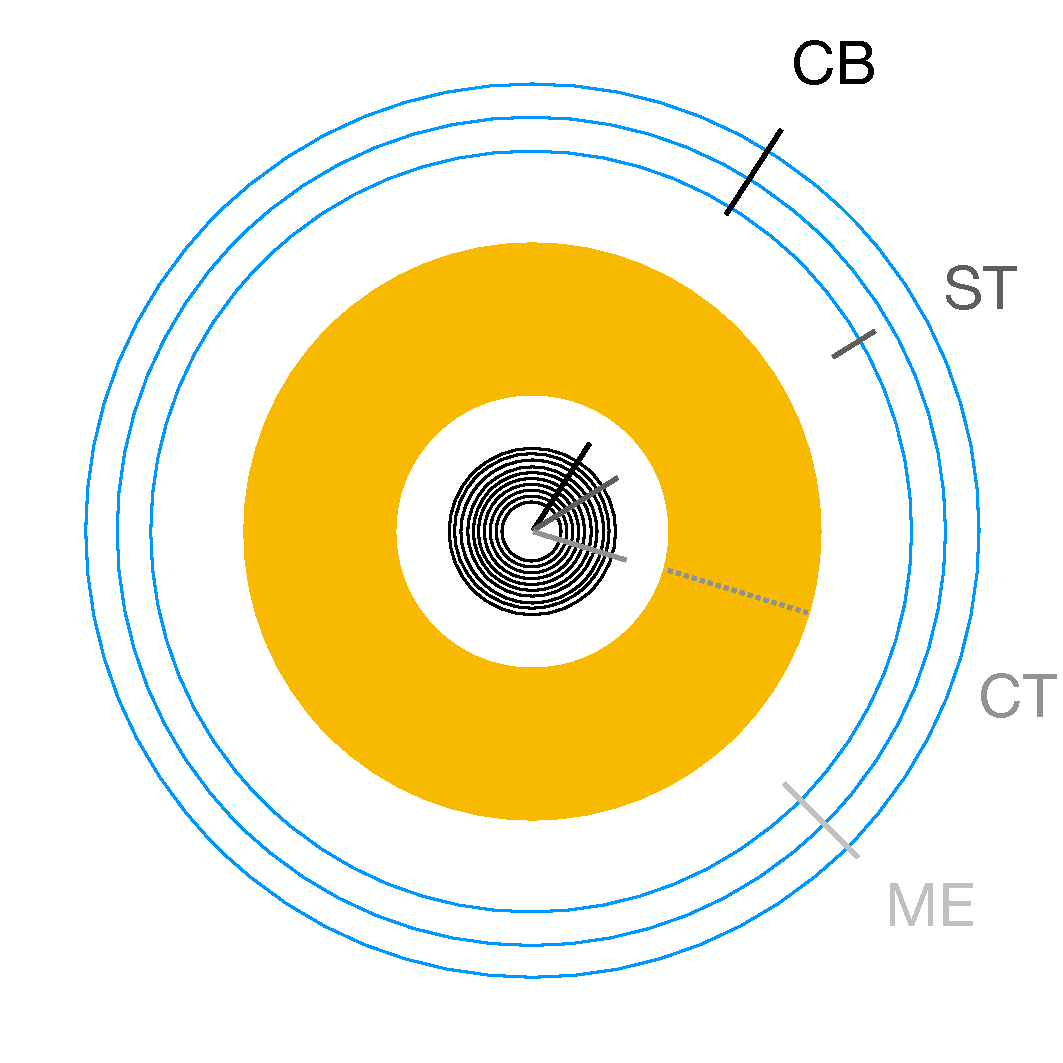
\includegraphics[width=0.5\textwidth]{Figures/LHC/muon_types.pdf}
    \caption{Cross-sectional view of the ATLAS detector and how muon types are identified. The inner black lines represent the inner detector, the yellow is the calorimeter, and the outer blue lines are the muon spectrometer. This figure is adapted from~\cite{Ottersbach:2012mma}.}
    \label{fig:typesofmuons}
\end{figure}
\subsubsection{Muon identification}

Muon identification is carried out with a cut-based approach \cite{ATLAS_muon_reco_2010}. The main backgrounds coming from hadron decays (mostly charged pion and kaon decays) are suppressed by applying quality requirements that select for prompt muons with high efficiency that provide robust momentum measurements. 

There are three identification variables used in discriminating a prompt muon from a background muon. These are:
\begin{itemize}
    \item the q/p significance, $\dfrac{q/p}{\sigma}$, the absolute value of the difference between the muon's charge to momentum ratio as measured in the inner detector and the muon spectrometer, divided by the total corresponding uncertainties;
    \item $\rho'=\dfrac{\p_{\text{T}}^{\text{ID}}-\p_{\text{T}}^{\text{MS}}}{\p_{\text{T}}^{\text{CB}}}$, the absolute value of the difference between the transverse momentum measurements in the inner detector and the muon spectrometer, divided by the transverse momentum of the combined track;
    \item the nomalized $\chi^2$ of the fit of the combined track.
\end{itemize}
Together these variables are sensitive in filtering out candidates from charged hadron in-flight decays in the inner detector. These have a topological "kink" that results in a combined track with poor fit quality, and incompatible momentum measurements coming from the inner detector and muon spectrometer. 

Various identification criteria are employed to target the diverse needs of physics analyses. Just like electron identification, the Loose, Medium, and Tight muon identification working points define progressively more restrictive requirements. Unlike the electrons, however, these working points differ not in the thresholds of a likelihood. Rather, they differ in the type of candidate muons permitted and in the requirements on the three variables defined above. 

The Loose identification criteria are chosen for the ATLAS work of this thesis, where all four types of reconstructed muons are used. The calorimeter tagged and segment tagged muons are restricted to a smaller region of $|\eta|<0.1$. This working point is designed to maximise reconstruction efficiency all the while providing good-quality tracks \cite{ATLAS_muon_reco_2016}. They were specifically optimised for an ATLAS Higgs analysis in the four-lepton final state \cite{ATLAS_H4l_2015}.  

\subsubsection{Muon isolation}

Just like electrons, muons have additional isolation requirements imposed to reject background, because muons originating from vector boson decays are often isolated while those originating from semileptonic decays are often embedded in jets. The activity around a muon candidate is therefore measured, in a similar manner  to that of the electrons, by summing a cone of transverse momentum and transverse energy in the tracking detector and calorimeter respectively. 

The tracking isolation is $p_{\text{T}}^{\text{varcone30}}$, defined as the scalar transverse momenta sum of tracks with $p_{\text{T}}>1$ GeV in a cone of size $\Delta R=\text{min}\Big(\frac{10}{p_{\text{T}}^{\mu}},0.3\Big)$ around the muon candidate. The contribution from the muon track itself is subtracted. The variability in cone size is to ameliorate performance for high $p_{\text{T}}$ muons \cite{ATLAS_muon_reco_2016}. Likewise, the calorimeter isolation variable, $E_{\text{T}}^{\text{topocone20}}$, is the sum of the topological energy clusters in a $\Delta R=0.2$ cone around the muon, with the energy deposit of the muon and pile-up effects subtracted. Various definitions for the discriminant variables are used to setup different working points. For the four lepton analysis, the FixedCutLoose working point is chosen, with $p_{\text{T}}^{\text{varcone30}}/p_{\text{T}}^{\mu}<0.15$ and $E_{\text{T}}^{\text{topocone20}}/p_{\text{T}}^{\mu}<0.30$. The details of the various muon isolation working points can be found in reference \cite{ATLAS_muon_reco_2016}.

% \cite{ATLAS:2020xtq}

